\section{Formulation of the problem}
\label{Formulation}
%==========================

\indent The primary goal is to deliver a payload, such as an egg to some height unharmed using a robot that is bio-inspired. The problem is broken up into two parts. The first part is to find a way to rapidly ascend updward. The second part is to implement a \textit{reasonable} deceleration. These two subproblems use two different mechanisms, one inspired by the flea for take-off and one inspired by the hummingbird for landing.\\

%===================== Trajectory ==========
\begin{figure}[H]
\begin{center}
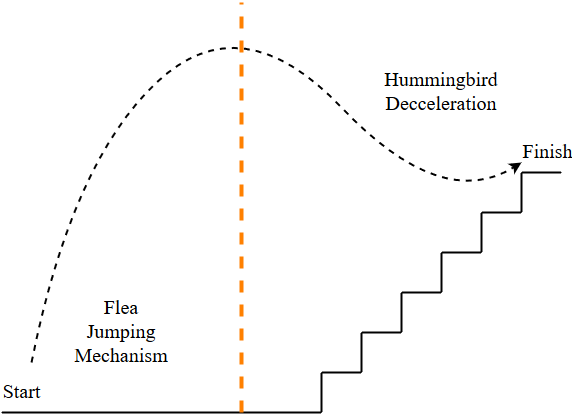
\includegraphics[width=0.75\linewidth]{./_Figures/trajectory.png}
\label{fig:trajectory}
\caption{This is a visual representation of the goal of delivering an egg to the top of a staircase. The orange line separates the two different mechanisms into their respective roles for the trajectory of the payload.}
\label{fig:trajectory}
\end{center}
\end{figure}
%===================== Trajectory ==========

\subsection{Acceleration Mechanism}
\indent As shown in \textbf{Figure} \ref{fig:trajectory}, the jumping mechanism will be used to achieve substantial height for the payload delivery. In order to draw inspiration from how a flea uses its energy to jump so high, energy usage will be explored in relation to payload mass as well as maximum height. A flea can jump many times its own height, but it is small in mass, approximately 45mg \cite[p.~63]{Bennet:1967}. Fleas have a ratio of mass to jump height and energy density. For a larger robot, a similar ratio could be achieved if energy density is proportionally higher to account for the larger mass. The larger mass is in part introduced by the need to carry an egg, which a flea does not have.\\

\indent It should be noted here that there is no path planning associated with the jumping mechanism. There may be an initial jump angle relative to the ground, but guiding the egg to the desired location is dealt with in the second part of the robot design. The proposed design for the jumping mechanism is shown in \textbf{section} \ref{implementation}.\\

\subsection{Deceleration Mechanism}
\indent This second part of the problem is associated with the bio-inspiration of a hummingbird. Hummingbirds are able to rapidly decelerate from specifically a diving trajectory. Assuming a substantial height is reached, this deceleration mechanism will be deployed to guide the egg to it's desired location safely. Wings will be used to realize this behavior. The design for this is shown in \textbf{section} \ref{implementation}.\\ 

